\documentclass[conference]{IEEEtran}
%\documentclass[10pt,sigconf,letterpaper]{acmart}

%\renewcommand\footnotetextcopyrightpermission[1]{} % 
%removes footnote with conference info
%\setcopyright{none}
%\settopmatter{printacmref=false, printccs=false, 
%printfolios=false}
%\pagestyle{plain}


\usepackage{color}
%\usepackage[nolist]{acronym}
%\usepackage{amsmath,amssymb}
\usepackage{pifont}
%\usepackage{enumitem}
\usepackage{booktabs}
\usepackage{url}
\usepackage{xcolor}
%\usepackage{times}  % Times fonts look better
\usepackage{array}  % Extended styles for tables
\usepackage{textcomp}
\usepackage{cite}
\usepackage{amsmath,amssymb,amsfonts}
\usepackage{algorithmic}
\usepackage{graphicx}
\usepackage{textcomp}
\usepackage{caption} 
\captionsetup[table]{skip=10pt}
\def\BibTeX{{\rm B\kern-.05em{\sc i\kern-.025em b}\kern-.08em
		T\kern-.1667em\lower.7ex\hbox{E}\kern-.125emX}}

% \iffalse
\iftrue
\newcommand{\randall}{\ding{110}\ding{43}\textcolor{magenta}}
\newcommand{\pes}{\ding{110}\ding{43}\textcolor{blue}}
\newcommand{\geoff}[1]{\ding{110}\ding{43}\textcolor{violet}{#1}}
\else
\newcommand{\randall}{}
\newcommand{\geoff}[1]{}
\fi

%\DeclareFontFamily{\encodingdefault}{\ttdefault}{\hyphenchar\font=`\-}

% \setcopyright{acmcopyright}
% \copyrightyear{2018}
% \acmYear{2018}
% \acmDOI{10.1145/1122445.1122456}

%\copyrightyear{2022}
%\acmYear{2022}
%\acmConference[IMC '22]{Internet Measurement 
%Conference}{October 25--27, 2022}{Nice, France}
%\acmConference{}{}{}
%\acmBooktitle{Internet Measurement Conference (IMC '22), 
%October 25--27, 2022, Nice, France}
%\acmPrice{TBA}

\begin{document}

\author{Anonymous Authors}
%\author{Audrey Randall}
%\email{aurandal@eng.ucsd.edu}
%\affiliation{UC San Diego}
%\author{Peter Snyder}
%\email{pes@brave.com}
%\affiliation{Brave Software}
%\author{Alisha Ukani}
%\email{aukani@ucsd.edu}
%\affiliation{UC San Diego}
%\author{Alex Snoeren}
%\email{snoeren@cs.ucsd.edu}
%\affiliation{UC San Diego}
%\author{Geoffrey M.\ Voelker}
%\email{voelker@cs.ucsd.edu}
%\affiliation{UC San Diego}
%\author{Stefan Savage}
%\email{savage@cs.ucsd.edu}
%\affiliation{UC San Diego}
%\author{Aaron Schulman}
%\email{schulman@cs.ucsd.edu}
%\affiliation{UC San Diego}
%\author{Wes Hardaker}

\title{The Challenges of Blockchain-Based Naming Systems for Malware Defenders}
%\renewcommand{\shortauthors}{A. Randall \textit{et al.}}

%\runningtitle{Article title}

%\subtitle{...}

\maketitle
\pagestyle{plain}

\begin{abstract}
	
Malware operators require the flexibility to change the 
location of C2 server in response to takedowns, without 
losing control of infected hosts. This flexibility requires a 

Malware requires a naming layer to contact its command 
and control (C2) servers, because infected hosts must have 
the flexibility to change where they expect the C2 server to 
be. Until recently, DNS domains were the obvious choice for 
implementing this naming layer, 
but DNS domains may be taken down by the registrar that 
sold them. Malware operators have recently responded to 
this threat by utilizing blockchain-based naming systems 
to store C2 server names. Blockchain naming systems are a 
threat for malware defenders because they are not subject 
to a centralized authority, such as a registrar, that can 
take down abused domains, whether voluntarily or under 
legal pressure. We analyze the blockchain naming system 
ecosystem and identify new locations for defenders to 
stage malware interventions. In particular, we find that 
malware is obligated to use centralized or 
semi-centralized infrastructure in order to connect to 
blockchain naming systems and modify their records. We 
also present a study of how blockchain naming systems are 
currently abused by malware operators, and discuss the 
factors that would cause a blockchain naming system to 
become an unstoppable threat. We conclude that
existing blockchain naming systems still provide 
opportunities for defenders to prevent malware from 
contacting its C2 servers.
\end{abstract}

\section{Introduction}

%\begin{itemize}
%	\item Malware, particularly botnets (any other types? ransomware?) 
%	uses DNS to reach CNC 
%	servers. 
%	\begin{itemize}
	%		\item Malware needs a naming layer because of the 
	%		sunk infrastructure cost: 
	%		any malware already deployed that uses an IP that gets 
	%blocked/taken 
	%		over is now useless. Malware authors want a record they can change.
	%		\item Naming layer needs to be hard to block at both 
	%		the request level and the system level, so that 
	%		already-distributed malware doesn't lose access and 
	%		become useless. 
	%	\end{itemize}
%	\item DNS is decentralized in that there are many resolvers, but 
%	centralized in that there are centralized authorities. Defenders can serve 
%	legal takedown notices to those centralized authorities to block malware's 
%	access to its CNC servers.
%	\item Pivot: Malware is starting to use a truly decentralized naming 
%	system, ``blockchain DNS.'' This creates several challenges for defenders:
%	\begin{itemize}
	%		\item No central authority is capable of enacting domain-level 
	%takedown 
	%		orders
	%		\item For large chains, there is enough legitimate content that 
	%		blocking access to the whole chain is infeasible
	%		\item Transactions on large chains cost a lot of money. This limits 
	%		defenders' abilities to stage interventions like pre-registering 
	%all 
	%		domains listed in a malware's DGA.
	%	\end{itemize}
%	\item We study the ecosystem and point out several places where 
%	interventions are still possible, and discuss the challenges to defenders 
%	and occasional advantages they gain when malware uses decentralized naming 
%	such as blockchain DNS.
%\end{itemize}

Malware that is distributed across multiple hosts 
needs a way to distribute 
commands, upload stolen 
data, and coordinate between infected machines. Most malware, 
such as botnets or 
ransomware, uses a 
central command and control (C2) server for this task. However, as a single 
point of failure, a 
central C2 server presents an obvious weak link for defenders to 
target~\cite{kesari_deterring_2017}. 
Malware authors must therefore be able to easily relocate and replace a C2 
server after a defender 
takedown. Furthermore, all previously infected hosts must be 
able to find the new server at 
its new address, 
without outside coordination --- if they cannot, they become useless. Malware 
authors avoid 
this ``sunk cost'' problem by providing a layer of 
indirection --- a \emph{naming 
layer} --- instead of 
hard-coding a fixed address directly into deployed malware. 
This 
naming layer must be 
resilient to takedown efforts.

Until recently, the naming layer used most frequently by malware was ordinary 
DNS, which is rarely 
blocked at the protocol level, universally supported, and easy to configure. 
Malware authors use 
various strategies, such as DGAs (domain generation 
algorithms), 
to cycle through domains and complicate defense efforts. 
However, 
DNS domains are subject 
to centralized authorities such as registrars, who may be 
compelled to 
seize or deny access to abused 
domains. Malware 
authors have recently come up with an innovative solution to this risk: they 
have started to use 
\emph{blockchain-based naming systems}. 

Blockchain naming systems present several potential 
challenges for 
defenders. First, because they 
have no central authority to carry out legal takedown 
requests, they are immune to one of the most effective tools 
in malware defenders' arsenals. Second, some blockchain 
naming systems 
have high transaction costs to register and manage domains, 
which renders some existing defense 
strategies ineffective. For example, registering all the 
domains 
that a DGA can generate 
is impractical in expensive blockchain naming systems. 
However, blockchain naming systems 
present challenges to malware authors as well, such as the 
difficulty of stealthily accessing the blockchain.

We study the blockchain naming ecosystem and point out 
several places where defender interventions are still 
possible. In particular, we argue that name resolution 
requests must 
pass through centralized or partially centralized 
infrastructure to access any blockchain naming system. These 
centralized ``chokepoints'' still present viable locations 
for defenders to stage interventions. We also study five 
existing 
blockchain-based naming systems, and discuss the challenges 
and advantages that each present to malware authors and 
defenders. 
\randall{we perform a measurement study of multiple major naming systems on how 
malware is currently them and conclude that some systems are used and others 
are not. Make another paragraph?}
We conclude that while blockchain 
naming systems present a significant threat, defenders still 
have viable options for enacting C2 takedowns.

%The remainder of this paper is organized as follows. 
%Section~\ref{sec:background} describes how malware currently 
%uses DNS domains to contact C2 servers, how defenders 
%stage interventions against these domains, and how blockchain 
%naming systems render these interventions ineffective. 
%Section~\ref{sec:naming_systems} gives an overview of the 
%five most widely adopted blockchain naming systems. 
%Sections~\ref{sec:accessing_records} describes where defenders 
%can intervene in malware's attempts to access naming systems 
%and control naming records. Section~\ref{sec:case_studies} 
%lists several case studies of interventions against 
%blockchain names and their 
%lessons for defenders. Section~\ref{sec:b-root} details how 
%blockchain naming systems are used by 
%malware today. Section~\ref{sec:discussion} discusses the 
%theoretical requirements for a naming system to be a threat, 
%Section~\ref{sec:related} presents related work, and 
%Section~\ref{sec:conclusion} concludes.
\section{Background}

From a malware author's perspective, an ideal naming system for C2 
addresses must be uncensorable at both the request level and the system level. 
To be 
uncensorable at the request level, there should be no central authority that 
has the ability to enforce a legal takedown notice for an individual record. To 
be uncensorable at the system level, the system should be valuable enough to 
licit actors that authorities cannot block access to it entirely without 
causing significant collateral damage to benign users.

To some extent, a trade-off exists between these features. On 
one side of the 
spectrum, protocols like Tor provide high resistance to request-level 
censorship, but they stand out in network traffic, allowing systems like 
IDSes to detect the 
malware's presence. For example, enterprise networks often block Tor 
entirely under the assumption 
that none of their employees will use it for any legitimate purpose.
%but do not have enough licit traffic to prevent authorities from 
%blocking access to the system entirely. \randall{Cite that paper that   
	%said when you take away the malware, what's left is 80\% CSAM, and find 
	%other 
	%citations that say defenders block Tor.}
On the other side of 
the scale, malware has repurposed ubiquitous, benign systems 
such as social media to store C2 addresses. Defenders do not 
want to impose blanket bans on applications accessing social 
media URLs, but social media companies such as Facebook and 
Twitter have the capability, motivation, and legal obligation to enforce 
legal takedown requests on individual posts. Malware authors want to use 
systems that are balanced 
between being difficult to block at the record level and difficult to detect 
and block at the 
system level.

\subsection{DNS-based domain names}

Traditional DNS has high system-level resistance to censorship but low 
request-level resistance. 
Since nearly every device and application on the Internet requires DNS, 
enterprises and firewalls 
almost never block it entirely. However, while DNS is a decentralized 
system in terms of how its 
components are replicated across the globe, it is not decentralized in terms 
of authority. The 
registrar that sold a domain can be compelled to ``delete'' that domain or 
prevent it from being 
updated or transferred. 

The usual process for enacting a legal takedown in the United States works as 
follows~\cite{knight_domain_2015}. Upon 
identifying a domain that is being used as a C2 center, a law enforcement 
entity may choose to make 
an Acceptable Use Policy (AUP) complaint or may immediately seek a court order 
compelling the 
registrar to take down the domain. Some registrars cooperate with AUC 
complaints without legal 
intervention, but others do not. If the registrar does not respond to the 
AUC complaint and take 
down the domain, law enforcement may move on to using a court order. The 
court order commonly 
prevents the domain from being updated or transferred rather than deleting it 
entirely, because if 
the domain is deleted, it can be re-registered by the malware authors. The 
court order also 
specifies whether the domain should continue to resolve, resolve to a new IP 
address specified by 
the order, or stop resolving altogether. 

Court orders may be obtained by civil parties as well. The most common method 
is for a company to 
apply for a temporary restraining order (TRO), which orders the perpetrators 
of the offending 
activity to cease and desist and requires any intermediaries that provide 
services to the 
perpetrators to cease providing those services~\cite{kesari_deterring_2017}. 
The latter requirement 
is what allows companies to require registrars to ``sinkhole'' C2 
domains. 

Legal domain takedown orders are a critical tool for defenders to disable 
botnets. For example, 
Microsoft obtained various court orders allowing it to sinkhole the C2 servers 
of the botnet 
Citadel in 2013. Microsoft successfully argued that Citadel caused the Windows 
operating system to 
behave maliciously and frustrate users while still bearing Microsoft 
trademarks, as well as forcing 
Microsoft to spend money on security features to combat 
it~\cite{lerner_microsoft_2014}. The 
Coreflood, Kelihos, and Rustock botnets were each disabled using legal 
takedown orders obtained by 
Microsoft, Pfizer (which claimed to suffer reputational harm because Rustock 
sent spam emails for 
counterfeit pharmaceuticals), and the Department of 
Justice~\cite{kesari_deterring_2017}. These 
takedowns are possible because in each case, some centralized entity had 
control of the C2 servers' 
domain names, and thus had the capability to take them down when legally 
compelled to. Malware 
authors are thus incentivized to find naming systems that are not vulnerable to 
legal takedowns.  

\subsection{Blockchain-based domain names}

Blockchain-based naming systems present a potential threat 
because they claim to be immune to takedowns. No central authority 
controls blockchain domains in the same way that registrars 
control traditional DNS names. In general, it is not possible to modify or 
delete a record on a blockchain without controlling the record's private 
key. Once a domain has 
been registered, its ownership is passed to the purchaser, after which 
point even the company that 
sold it cannot modify it. The record is also stored immutably on the 
blockchain for as long as the 
chain exists, even if the owner later modifies or deletes it, because 
historical recods are part of 
the blockchain and cannot be erased. Blockchain-based naming systems 
therefore have high resistance 
to request-level censorship.

Furthermore, some blockchains are popular enough to be challenging to block 
without 
harming licit users. Blockchains such as Bitcoin and Ethereum have recently 
skyrocketed in popularity as investors became interested in cryptocurrency as 
an asset class. Because these blockchains are no longer niche systems used 
only by a few 
technologically-savvy users, blocking access 
to them entirely may be difficult without angering a large number of 
legitimate users. As far as we are aware, cryptocurrencies and the blockchains 
they rely on are the first examples of strongly censorship-resistant systems 
that have gained a substantial community of legitimate users around the world.

Blockchain is therefore an attractive option for malware authors to use as a 
naming 
layer for C2 server addresses. In fact, some malware is already exploiting 
these tools.
BazarLoader uses the Emercoin ``.bazar'' TLD to record the domains of its C2 
servers~\cite{brandt_bazarloader_2021}. The Namecoin TLD 
``.bit'' is used by the
Necurs botnet~\cite{dgas_of_necurs}, the Chthonic banking 
trojan~\cite{malware_traffic_analysis_2016}, Smoke Loader/Dofoil, 
Backdoor.Teamviewer, Shifu, 
and TinyNuke~\cite{abusech_2017, mackie_cryptodns_2018}. Cerber ransomware 
has 
even used blockchain wallet addresses as names for its C2 
servers~\cite{pletinckx_malware_2018}.

However, we find that blockchain domains are not as invincible as they 
claim. While sinkholing 
blockchain domains through their registrars is not possible, blockchain 
domains have two different 
weaknesses that DNS does not have: accessing the system and modifying records.

Blockchain domains are not accessible through traditional DNS. Instead, 
malware 
must find a way to contact a member of the blockchain to resolve its chosen 
domain. Malware authors 
can implement this in two ways: they can either use a centralized proxy with a 
known domain to gain 
access to the blockchain, or they can act as first-class participants of the 
blockchain themselves, 
and participate in the peer-to-peer discovery protocol. Both approaches 
present opportunities for 
defenders to intervene. 

Modifying records on blockchains also poses new challenges for both defenders 
and malware authors. 
Modifications are usually more expensive (in terms of money) than in DNS, 
making fast flux or DGA 
impractical on some chains. Similarly, if a defender wishes to register 
all domains that a DGA 
might produce, this becomes expensive on some chains.

In the remainder of this work, we detail the specific challenges posed by the 
blockchain DNS 
ecosystem to malware authors and defenders, as well as the pieces of the 
ecosystem where 
effective interventions might be staged.
\section{Specific naming systems}
\subsection{General Purpose Naming Systems}

Interestingly, systems like ENS and Unstoppable Domains are not advertised as 
drop-in replacements for DNS. Rather than being intended specifically to 
resolve to IP addresses, these naming systems often translate a human-readable 
name to a \emph{wallet address} instead. While users can still store IP 
addresses, very few choose to do so. \randall{need numbers here or later in 
	specific chain section}. Some users store the addresses for distributed 
	storage 
systems, but the majority of configured records store wallet addresses. We also 
note that a high percentage of names on ENS and Unstoppable Domains are not 
configured to have records at all. There may be a few reasons why: first, names 
resolve to the wallet address that owns them by default \randall{true on 
	Unstoppable?}, which may be the only use some customers require. Second, 
	while 
purchasing a domain is very straightforward and only requires using a website, 
adding a record requires interacting with smart contracts on the blockchain, 
because only the owner of the domain may modify its records. The company that 
sold the domain no longer has the ability to add records for the user unless 
the user chooses to park their domain in the company's wallet-hosting service. 
This requirement is not obvious at the purchasing step. Third, a large number 
of names appear to be purchased as speculative assets rather than because users 
wish to utilize them directly. 

We now describe the workings of two Ethereum-based naming systems: the 
Ethereum Name Service (ENS) and Unstoppable Domains. 
\subsubsection{ENS}

\begin{table}
	\begin{tabular}{lrr}
		\toprule
		Resolver Name & Txns that Set this Resolver & Address \\
		\midrule 
		Public Resolver 2 & 33,304 & \texttt{0x4976fb...} \\
		Public Resolver 1 & 2,736 & \texttt{0xDaaF96...} \\
		OpenSea ENS resolver & 482 & \texttt{0x9C4e9C...} \\
		ENS Old Public Resolver 2 & 440	& \texttt{0x226159...} \\
		Umbra: Stealth Resolver & 409 & \texttt{0xB37671...} \\
		\textit{unnamed PublicResolver} & 126 & \texttt{0xD3ddcC...} \\
		\textit{unnamed PublicResolver} & 103 & \texttt{0x5FfC01...} \\
		ENS Old Public Resolver 1 & 29 & \texttt{0x1da022...} \\
		\bottomrule
	\end{tabular}
	\label{tab:ens_resolvers}
	\caption{The ENS resolvers from which we collected a sample of names and 
		records.}
\end{table}

\begin{figure}[t]
	\centering
	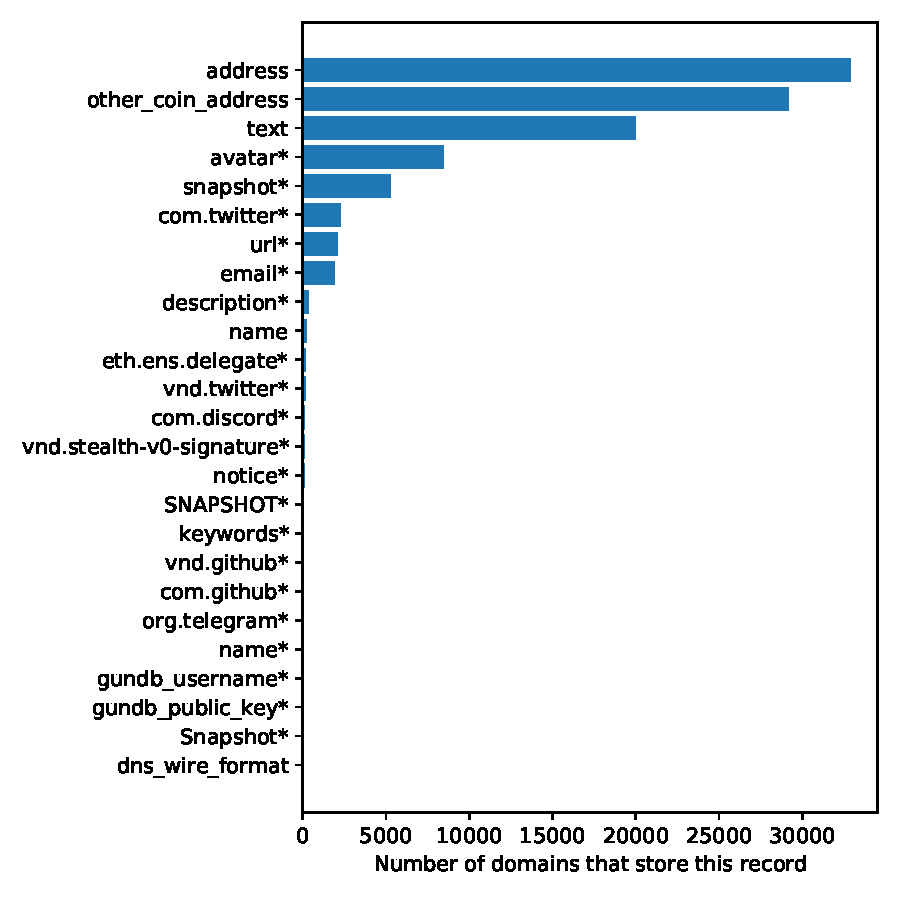
\includegraphics[width=3in]{figs/ens_names.pdf}
	\caption{Records stored by ENS names. *key within ``text'' record}
	\label{fig:ens_records}
\end{figure}

ENS names use smart contracts to fill the roles of the single registrar and 
multiple resolvers in the system. When claiming a name for the first 
time, the user sends a transaction from their wallet to the ENS Registrar 
Controller 
contract, requesting that the name be registered and transferred to the 
ownership of the wallet. The ENS Registrar Controller sets a number of default 
values, including a default wallet 
address record that maps the name to the wallet address that owns it, and a 
default resolver contract for the 
name, which at the moment is the ``ENS Public Resolver 2'' smart 
contract.\footnote{The public 
	resolver contract was updated in the past, and almost all ENS names have 
	now 
	changed their resolvers away
	from the ``Old'' resolvers, usually to the current default resolvers.} To 
	fully 
resolve a 
name, a user must first query the ENS Registrar Controller to determine the 
name's designated resolver, and then query that resolver for the record 
associated with the name. Resolver contracts are allowed to access the storage 
of the ENS Registrar Controller, which means they don't have to perform another 
transaction for the resolver to know that a new record has been created by the 
ENS Registrar Controller. 

Users cannot query a resolver for a name's records directly: they must first 
convert the name to its keccak256 hash. These 
name hashes are referred to as ``nodes.'' Because keccak256 hashes are not 
reversible, 
translating a node back to a name is a non-trivial process. Some name owners 
choose to register their node-to-name mapping in the ``ENS Reverse Registrar'' 
contract, but this practice is not required. While it is possible to enumerate 
all of the transactions that recorded new names from the Registrar Controller 
Contract (and its historical predecessors, such as a contract that was used to 
register short names earlier in ENS's lifetime), this approach still yields some
nodes for which names were never recorded. 

requires another contract, the ENS Reverse 
Registrar. Names are not required to have entries in the ENS Reverse Registrar, 
so this contract is not always able to translate a given node 
back to a name. 

One more notable feature of ENS names is that anyone may renew 
them, not just their owners. The reason for this design choice 
is unclear.

To study this ecosystem, we took a sample of names from the eight resolver 
contracts that were set by the most names as their default resolver. We chose 
eight because the distribution of resolvers is long-tailed: the majority of 
resolvers resolve only a few names, while the eight most popular resolvers 
resolve the majority of names. We excluded addresses that were set as resolvers 
by many names but did not implement the ENS resolver specification, under the 
assumption that these were mistakes. Such misconfigured resolver addresses 
include the null address, 
0x0, as well as other smart contracts used by the ENS ecosystem, such as the 
``Base Registrar Implementation.''  The remainder of the resolvers we chose are 
detailed in Table~\ref{tab:ens_resolvers}.

At the time that we performed this study, 667,369 ENS names had been 
registered through the Registrar Controller contract. Names that did not 
specify a resolver when they were registered 
were assigned the default ENS Public Resolver 2, which presumably accounts for 
the vast majority of the names that never performed an explicit transaction 
setting their resolver. \randall{I'm in the middle of checking this.} 

Figure~\ref{fig:ens_records} shows the distribution of the types of records 
stored by our sample of names. The majority resolve to wallet addresses or text 
records, not IP addresses, traditional domains, or DS addresses. We broke down 
the text records, which are key/value pairs, by the most common key names: 
these keys are marked with an asterisk. Only the most common 25 keys are shown. 
We note that only 17 names had \texttt{dns\_wire\_format} records, which are 
intended to store traditional DNS 
records, and all 17 are malformed as far as we can tell. \randall{should maybe 
	work on that some more? Couldn't tell what was wrong by examining the 
	octets.}

%Describe the registrar/registry/resolver structure. We took a sample 
%of X domains from the most 
%frequently updated resolver contracts.
%
%Haven't found anything bad yet except loli-hentai.x. This 
%system, like all other uncensorable systems, will probably 
%eventually attract CSAM. Describe what we did to find 
%domains, how I crawled a subset.

\subsubsection{Unstoppable Domains}

\begin{figure}[t]
	\centering
	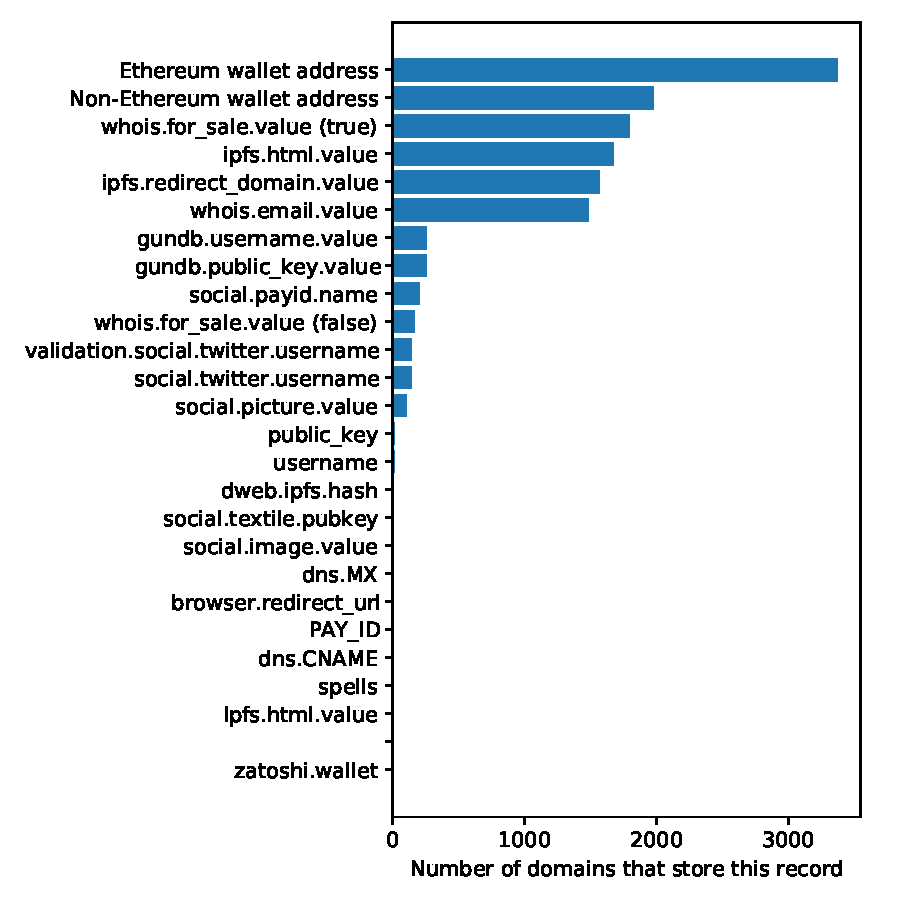
\includegraphics[width=3in]{figs/all_unstoppable_records.pdf}
	\caption{Records stored by Unstoppable Domains names.}
	\label{fig:unstoppable_records}
\end{figure}

%Describe the registry contract and the crawled domains (I did 
%crawl these didn't I?)

Like ENS, Unstoppable Domains uses Ethereum smart contracts as 
registrars. Unstoppable names are divided into two systems. CNS 
(Crypto Name System) contains all names with \texttt{.crypto} 
TLDs, and has separate registry and resolver contracts. This 
system was created first. Later, Unstoppable added UNS 
(Unstoppable Name System), which simplified name resolution by 
combining the resolver and registry contracts, and added several 
new TLDs. Unstoppable names never have to be renewed; they are 
purchased once and then owned for life. This is primarily 
because Unstoppable Domains does not have the capability to 
reclaim a name unless the private key of the owning wallet is 
known to them. 

Unstoppable names are referenced by their namehashes, which are 
similar to ENS's ``nodes.'' We extracted all namehashes from the 
Unstoppable Domains registry contract by searching all of its 
transactions, and then found each name's records by querying 
Unstoppable's metadata endpoint.\footnote{
	\texttt{https://metadata.unstoppabledomains.com/metadata/}} 
Figure~\ref{fig:unstoppable_records} shows the 
distribution 
of record types found in the Unstoppable Domains names. As in 
ENS, the majority of names have wallet records rather than 
records that point to websites in any way. The next most common 
type of record is ``whois.for\_sale.value,'' showing that many 
names are seen as speculative assets. Unstoppable Domains also 
provides an easy way for users to link to IPFS records. IPFS, 
the ``Inter-Planetary File System,'' is a distributed 
blockchain-based hosting service that allows users to host 
static websites.

We performed a web crawl of all of the Unstoppable names that 
had records pointing to websites, whether IPFS records, 
traditional IP addresses, or traditional domains. We took 
screenshots of the 367 websites we arrived 
at, inspected them manually, and did not find any evidence of 
malware use. Most 
websites were personal sites, Web3-based business sites, or related to the sale 
or collection of NFTs. 

We also examined the sample of names from B-root for any Unstoppable Domains 
names that appeared to be associated with malware. 

Unstoppable Domains has claimed that their naming system is not well suited for 
malware authors or other miscreants for two reasons. First, Unstoppable Domains 
claims to police which domains may be sold. The CEO of Unstoppable Domains, 
Matthew Gould, stated in an email that Unstoppable ``prevented the 
registration of domains associated with known pirating software or other types 
of IP theft and fraud''~\cite{pegoraro_blockchain_2021}. Second, Unstoppable 
can also seize a domain if that 
domain is hosted by Unstoppable's custody 
wallet, instead of by a private wallet~\cite{pegoraro_blockchain_2021}. In 
fact, other wallet hosting 
services, such as Coinbase's, 
could presumably also seize wallets that store domains, since the private 
keys of those wallets are 
known to the service. However, we note that seizing hosted wallets may not 
be a reliable 
intervention, because malware authors can evade this tactic by simply using 
self-hosted wallets. 

\subsection{Naming-Specific Blockchains}
\subsubsection{Namecoin and Emercoin}
\subsubsection{Handshake}
\begin{table}
	\begin{tabular}{lr}
		\toprule
		Record & Names with Record \\
		\midrule
		Default NS and GLUE4 records & 102,386 \\
		\hspace*{0.2in} No A records & 102,285\\
		\hspace*{0.2in} A 44.235.163.135 & 94 \\
		\hspace*{0.2in} A 52.43.158.89 & 4 \\
		\hspace*{0.2in} A 144.91.114.245 & 2 \\
		\hspace*{0.2in} A 1.1.1.1 & 1 \\
		Invalid name & 98,068 \\
		No record (null) & 845 \\
		TXT record & 138 \\
		\hspace*{0.2in} ``hello fx-wallet'' & 110 \\
		\hspace*{0.2in} Other & 28 \\
		Non-default NS record & 32 \\
		Non-default GLUE4 record & 11 \\
		Distributed storage address & 7 \\
		\midrule
		Total unique names & 201,458 \\
		Total records & 201,487 \\
		\bottomrule
	\end{tabular}
	\caption{Record types in the Handshake namespace.}
	\label{tab:handshake_records}
\end{table}

Handshake is a new blockchain-based system that aims to 
replace the root DNS 
zone. As such, it offers its users the ability to purchase 
nearly any string to 
use as a TLD. Rather than selling second-level domains 
itself, the Handshake ecosystem purports to allow its users 
to act as registrars who can sell their own domains. 
Handshake's stated goal is not to replace the traditional DNS 
system: Handshake records are designed to store the domains 
and IP addresses of traditional authoritative nameservers, 
rather than to store A, AAAA, or CNAME records. However, we note that nothing 
restricts malware authors from recording the IP addresses of C2 servers as NS 
records, or running an authoritative nameserver and a C2 server on the same 
machine. Handshake also allows users to store TXT records, which can 
contain the addresses for decentralized web hosting systems 
like Skynet or IPFS. Malware users could potentially use 
Handshake as a naming system to find content stored in 
content-addressed distributed storage systems. Additionally, Handshake 
advertises themselves as ``the only naming blockchain with a lightweight 
recursive DNS resolver, which you can easily embed into 
browsers, apps, and devices''~\cite{namebase_access_handshake}. 
This lightweight resolver may be attractive to malware authors because it is 
small enough to use as part of a malware payload.

We collected a sample of approximately 201,000 Handshake names and analyzed the 
records assocated with them. Table~\ref{tab:handshake_records} 
summarizes our findings. At the moment, Handshake names appear to be 
overwhelmingly used as speculative assets. Only 0.14\% of names in our sample 
had records that led to either IP addresses or DS addresses, assuming the 
non-default nameserver and glue records do lead to IP addresses or DS 
addresses. Nearly half of registered Handshake domains in our sample cannot be 
resolved by the HNS client, since they contain illegal characters like emojis 
or are solely composed of numbers: these names are nevertheless allowed to be 
minted.

Because these names seem to have very few records and we can't look them all 
up, we don't pay Handshake much attention from here on out.
\section{Intervention Locations}
\label{sec:accessing_records}

\begin{figure*}[t]
	\centering
	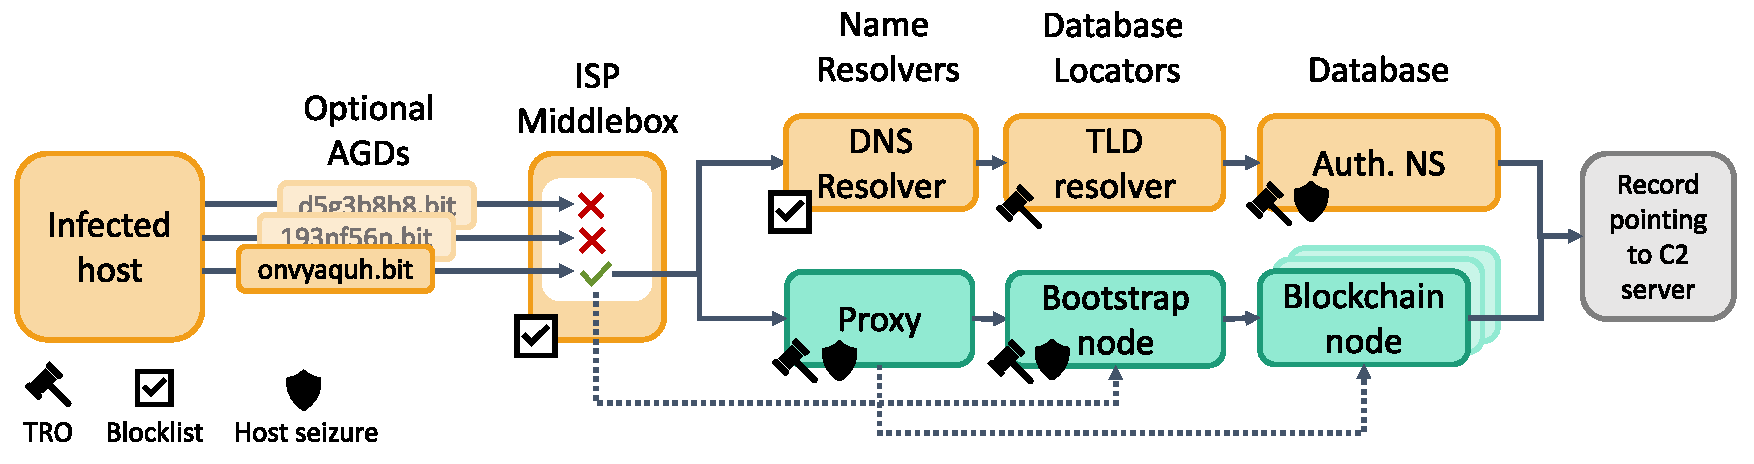
\includegraphics[width=\textwidth]{figs/intervention_locations.pdf}
	\caption{Potential locations of interventions for 
	blocking access to DNS-based and blockchain-based C2 
	server names.}
	\label{fig:malware_contacting_cnc}
\end{figure*}

We have established that malware requires a naming layer to access its C2 
centers, and 
that blockchain-based naming systems are attractive options for implementing 
such a naming layer. We have also examined five naming 
systems individually. 
We now argue that all blockchain-based naming systems share 
certain common 
challenges, and the way these systems overcome these challenges presents 
different advantages or disadvantages for defenders. The first 
of these fundamental challenges is accessing the blockchain.

Accessing any distributed, peer-to-peer system for the first time requires 
learning the address of at least one participating node. In general, there 
are two methods for finding such an address: connecting to a 
proxy that already knows how to reach a member of the system, or acting 
as a full member of the system and utilizing its peer-to-peer discovery 
protocol. The latter approach requires knowing a list of ``bootstrap nodes.'' 
For example, Ethereum uses a list of bootstrap nodes that are hard-coded into 
client implementations~\cite{geth_bootstrap}. Bitcoin 
stores lists of bootstrap nodes in DNS TXT records maintained by volunteers, as 
well as hard-coded 
lists~\cite{bitcoin_bootstrap}. A third option, a 
local discovery protocol that floods the network with 
messages looking for nodes, has not been adopted by any 
blockchains that we are aware of. Such an approach would only be successful if 
nodes running the blockchain were present on most networks. 
 
Figure~\ref{fig:malware_contacting_cnc} compares the steps an infected host 
takes to resolve a DNS C2 domain to the steps required to resolve a blockchain 
name. It also details the interventions that can be taken by defenders at each 
step. We now describe each step in detail.

\subsection{Reaching the resolver}

Regardless of whether a request is destined for DNS or a blockchain naming 
system, it must first reach the machine that acts as a resolver: either the DNS 
resolver or the proxy in Figure~\ref{fig:malware_contacting_cnc}. Defenders may 
be able to intervene before this point by placing middleboxes with filter lists 
in the network. Some networks already have such defenses: for example, some ISP 
networks redirect all DNS requests to the ISP's own resolver, which can 
implement a filter list. This defense is probably not currently intended to 
block blockchain names, but it works by chance in some cases. Some malware uses 
ordinary DNS rather than DNS-over-HTTPS to request blockchain domains, under 
the assumption that the proxy the query is intended for will redirect it to the 
blockchain naming system in the correct format. When ISPs perform DNS 
redirection to their own resolvers, these queries get redirected to the DNS 
root, which cannot resolve the alt-TLDs used by blockchain naming systems. We 
present our study of this phenomenon in Section~\ref{sec:b-root}. We observe 
that filter lists are only a partial defense against malware, because malware 
may utilize DGAs to evade them. 

\subsection{Interventions at the name resolver}

When using blockchain naming systems, the entity that first attempts to resolve 
a request is a proxy rather than a pure DNS resolver. It may expect queries in 
the form of DNS-over-HTTPS, unencrypted DNS, or in an 
arbitrary format. Instead of querying the DNS root zone, the 
TLD resolver, and eventually the authoritative nameserver to 
resolve a name, the proxy must connect to the blockchain and 
retrieve the record from one of the participants.
Defenders may intervene at a traditional DNS resolver by requesting that the 
resolver implement a filter list, or the resolver operators may elect to 
implement one voluntarily. However, proxies that resolve blockchain names may 
be resistant to such voluntary efforts, because proxy 
operators often identify with the libertarian values 
associated with the goals of blockchain. 


Proxies are currently the most common method for resolving 
blockchain names. Table~\ref{tab:proxies_and_tlds} shows a 
selection of the proxies and tools that resolve names from 
each of the systems we study. The list of proxies is not 
exhaustive, but represents 
a subset of the best-known proxies in use at the time of 
writing. While most large 
browsers, such as Safari, Chrome, and Firefox, do not support 
any blockchain naming systems natively, some naming systems 
provide browser extensions that redirect blockchain name 
queries to proxies using DoH. A few browsers do resolve 
blockchain names without requiring extensions, such as Brave, 
which partners with a proxy called 
Infura~\cite{brave_uses_infura}. Some naming systems have 
partnerships with existing DNS resolvers. For example, 
NextDNS's DNS resolvers can act as proxies to resolve 
Handshake names. Finally, some naming systems, such as 
Handshake, also provide stub resolver implementations that 
run locally on a user's computer. These stub resolvers also 
work by routing blockchain name queries to proxies.

All of these proxies are centralized, in that they 
are controlled by a single authority. This is good 
news for defenders: similarly to traditional registrars, they 
are vulnerable to legal takedowns. They can be served with 
TROs or warrants and compelled to stop giving access to 
abused domains, as long as they operate within a jurisdiction 
amenable to such efforts. A centralized proxy could also be 
neutralized by serving a takedown order to its 
hosting provider, although this approach would produce 
varying amounts of the collateral damage depending on how 
many licit users utilize the proxy. 
While these interventions are not 
foolproof, they are subject to the same advantages and 
disadvantages as interventions on traditional registrars. 
Thus, centralized proxies return the distributed naming 
ecosystem to a state similar to the DNS ecosystem, from a 
defender's point of view. 
%We conclude that proxy takedowns 
%are a viable method for 
%defenders to intervene in the blockchain DNS ecosystem. 
However, while proxies greatly simplify the process of 
connecting to a blockchain, they are not strictly necessary, 
which is bad news for defenders.

\subsection{Skipping the proxy: the rise of light clients}

We initially assumed that no infected host would be able to 
skip the proxy and participate directly 
in the blockchain, because acting as a blockchain node 
requires too many resources. However, this assumption turned 
out to be incorrect, because of the rise of \emph{light 
clients}. When blockchains were first envisioned, most 
assumed that every participant in the network would be a 
``full'' implementation of a node: it would contain 
enough state to reconstruct the entire history of the chain, 
all the way back to the first transaction. Additionally, each 
node would contribute to the 
blockchain by verifying every transaction it heard about. As 
blockchains grow over time, they become too 
resource-intensive to run on anything other than a dedicated, 
powerful machine. Two resources serve as 
the constraints: first, CPU power, which is obviously 
necessary to perform mining but now is even a bottleneck for 
transaction verification, because so many transactions happen 
per second~\cite{citation_needed}. Second, disk 
space and speed. For example, a full Ethereum node cannot be 
run on a machine with a hard disk drive anymore, because 
nothing slower than an SSD can keep up with the 
reads and writes required~\cite{citation_needed}. These 
resource constraints make it 
very unlikely that malware could run ``full'' blockchain 
nodes on infected hosts. However, these constraints have also
given rise to the concept of a ``light client,'' a blockchain 
node with limited functionality that can fetch transactions 
from the chain but does not contribute by verifying 
transactions, mining, or broadcasting. Light clients are 
designed to run on laptops and mobile devices. As such, they 
use few enough resources to reasonably be included in 
malware. 


\subsection{Interventions at the Database Locator}

Light clients enable malware to act as a first-class member 
of a blockchain, and discover other members of the chain 
using the chain's peer-to-peer discovery protocol without 
using a centralized proxy. In this case, defenders are left 
with a harder location to stage an intervention: the 
blockchain's bootstrap nodes, which is the blockchain 
equivalent of a service that locates the database of naming 
records.

%Most peer-to-peer discovery 
%protocols allow a client to connect to the blockchain for 
%the 
%first time by hard-coding a set of ``bootstrap nodes.'' In 
%Ethereum, these bootstrap nodes are hard-coded into various 
%implementations of the clients, and in Bitcoin, they are 
%either hard-coded or accessible as TXT records stored at 
%various trusted domains. The list of bootstrap nodes may 
%also 
%be configured by the user. If the 
%malware chooses to use the bootstrap nodes that are 
%hard-coded by default into the light client implementation, 
%this may present a challenge for defenders, because taking 
%down those bootstrap nodes may cause collateral damage to 
%legitimate users attempting to join the chain. As such, 
%bootstrap nodes are a more difficult place to stage an 
%effective defender intervention than centralized proxies. 


In traditional DNS, the resolver must locate the database 
that contains a record by first querying the hierarchy of DNS 
servers: first the root and then the TLD resolver. The TLD 
resolver's role is to tell the DNS resolver which machine 
stores the database that ultimately contains a name's 
records. In a blockchain system, this role is filled by the 
blockchain's bootstrap nodes, which are publicly listed 
nodes that maintain connections to some of the other 
participants in the blockchain. The purpose of the bootstrap 
nodes is to provide a gateway to the blockchain for new 
participants: new blockchain nodes find their initial list of 
potential peers by connecting to the bootstrap nodes.

When defenders perform interventions by putting legal 
pressure on registrars, the intervention takes effect at the 
TLD resolver, which implements the changes to the zone file 
that affect the malware's domains. These changes can include 
``sinkholing'' the domain by causing it resolve to an IP 
controlled by defenders or ``freezing'' it so that 
its records cannot be modified. This intervention does not 
translate well to blockchain naming systems for several 
reasons. 

First, while bootstrap nodes are responsible for finding the 
entire naming database, they do not allow defenders to 
specify which blockchain systems a client may access and 
which it may not. This means that seizing a specific naming 
record, or even the entire naming system, is not possible at 
the bootstrap nodes. Consequently, disabling or seizing 
bootstrap nodes prevents all new clients from accessing any 
functionality provided by the blockchain, including the 
blockchain's cryptocurrencies and any services it offers 
unrelated to naming. This approach therefore carries the 
potential for a lot of collateral damage. Second, bootstrap 
nodes may be widely distributed across the globe, leading to 
jurisdictional challenges in bringing legal pressure to bear 
on their operators. Bootstrap nodes may also be difficult to 
find, since they may not be run by hosting providers but 
rather by anonymous individual volunteers. Third, bootstrap 
nodes may be numerous enough that finding and seizing them 
all may be prohibitively difficult. Finally, while the 
default bootstrap node lists are published for each 
blockchain, users may choose to substitute their own. A 
malware author could design a payload that contains an 
extensive list of machines that participate in a blockchain 
naming system, which would complicate a defender's efforts to 
take down all the potential participants. 

However, defenders could fall back to a blocklist-based 
approach to deny access to bootstrap nodes. For example, 
IDSes, enterprise firewalls, or ISP routers can drop traffic 
intended for bootstrap nodes. This approach is very similar 
to blocking any other 
malicious IP addresses, and is subject to the usual 
challenges. Defenders must keep blocklists up-to-date as 
malware authors update the IPs they connect to. To the 
advantage of defenders, any time malware authors 
are forced to update the IP addresses that bootstrap nodes 
may be found at, they run afoul of the ``sunk cost'' problem 
where infected machines that cannot be updated become
useless. A similar argument applies if malware chooses to 
access bootstrap nodes using hard-coded DNS domain names 
instead of hard-coded IP addresses. Additionally, 
traditional interventions against domain names apply in that 
situation as well. Thus, while intervening at bootstrap nodes 
poses more of a challenge than intervening at centralized 
proxies, defenders still have viable options to choose from.

\subsection{Interventions at the Database}

In traditional DNS, defenders can sinkhole the domain of an 
authoritative nameserver or seize the server itself to 
prevent malware accessing a C2 domain record. This 
intervention is impractical for blockchain names, 
because instead of a single machine acting as the 
authoritative nameserver, every blockchain node has a copy of 
the database. Seizing the database would require either taking down 
every machine in the blockchain, or executing a successful ``51\%'' attack by 
taking control of more than half of the computing power in the blockchain. 
Blockchains are generally highly robust against attacks like these, which makes 
them unlikely to be the most practical intervention for defenders to attempt. 
However, small naming-specific
blockchains with few participants may be more vulnerable --- see 
Section~\ref{sec:namecoin_51}.

\subsection{Interventions after the name record is acquired}
\label{sec:interventions_at_name}

If an infected host successfully retrieves its C2 record, 
that record might take several forms. The three that we 
observed in existing blockchain naming systems that might be 
useful to malware were IP addresses, traditional DNS domains, 
and addresses for distributed storage systems like IPFS and 
SkyNet. We refer to these addresses as ``distributed 
storage'' (DS) addresses from this point forward. Some naming 
systems also allow users to store arbitrary text as 
records, which would let malware operators store nonstandard 
record types like links to social media posts. 

Each of these record types are subject to all of the 
traditional interventions that have already 
been described, except one: DS addresses. Distributed storage 
systems provide a form of ``bulletproof'' hosting, under the limitation
that all hosted content must be static files and not dynamic 
websites. Any C2 server implemented entirely on such a 
system must be a simple file with no 
dynamic content. Infected hosts that wish to contact a distributed storage 
system must pass through the same steps shown in 
Figure~\ref{fig:malware_contacting_cnc} for accessing a blockchain, which means 
they are subject to the same interventions. For example, a strain of malware 
called ``IPStorm'' has already been discovered using IPFS for its C2 server in 
the wild. IPStorm connects to IPFS using bootstrap nodes~\cite{ipstorm_anomali, 
ipstorm_zdnet}, which may be seized or blocked.

Another advantage for defenders is that some distributed storage systems, 
such as IPFS, do not have redundancy: only a single machine hosts each piece of 
a file. This raises the possibility of discovering the particular machine 
responsible for hosting a C2 server and seizing it. 

A final possibility for intervening with the name record may be to seize 
names stored in ``hosted'' or ``custodial'' wallets. Businesses such 
as cryptocurrency exchanges provide custodial wallets for users who wish to let 
the company handle their blockchain-based assets. This service is designed to 
make blockchain interaction easier for customers, but as a consequence, the 
business knows the custodial wallet's private key. If a name is stored in a 
custodial wallet, the business that runs the wallet 
could seize it~\cite{pegoraro_blockchain_2021}. However, a 
successful intervention must be difficult for malware operators to 
evade, and we note that malware operators with good operational practices can 
simply choose not to use custodial wallets. 

\subsection{Intervening with name modification or purchase}

Generally speaking, DNS domains are cheaper, easier to modify, and 
easier to replace than IP addresses, because each IP address 
represents a compromised machine while new domains can be 
purchased inexpensively. Blockchain-based domains on 
general-purpose chains, such as Bitcoin and Ethereum, 
change this norm. While resolving a name is free, malware 
operators must pay \emph{transaction fees} 
(known as \emph{``gas fees''} on Ethereum)
to register or modify names. These transaction fees 
can be quite expensive. For example, we found that 
registering a new name on the Unstoppable Domains service 
cost nearly \$80 in gas fees during a period of high fees. 
In contrast, the cost of the name itself was \$10. While 
licit users may wait for fees to be low at times of low 
network congestion, malware operators may not have that 
choice if they wish to avoid downtime in their campaign. High 
transaction costs poses challenges for defenders as well. For 
example, to combat DNS-based DGAs, defenders have the option 
of registering every domain the DGA will ever generate. This 
intervention would be much less practical if each 
registration was nearly an order of magnitude more expensive.

Naming-specific blockchains, such as Namecoin, Emercoin, and Handshake, 
present a different set of tradeoffs for defenders and malware 
operators. These 
blockchains are created with the sole intention of hosting a naming system. 
With fewer users and correspondingly less demand, these systems' names are 
usually much less expensive than names in Ethereum-based systems. This enables 
malware authors to use fast flux or DGA-based strategies, and also may enable 
defenders to pre-register domains generated by DGAs. 






%\subsection{Naming record formats}
%
%
%
%
%\randall{where do I put this? Additionally, because all 
%blockchain 
%	records 
%	are public, anyone can fetch those records including 
%	defenders. You could theoretically scrape a blockchain 
%looking for records 
%	that match a known 
%	malicious format or with malicious traits of some sort 
%(owned by the same 
%	wallet?) and try to seize 
%	whatever those records point to.} 
%
%
%
%I don't know if IPFS/SkyNet have light nodes that could be 
%part of a malware payload, but there does seem to be a trend 
%in that direction as chains get heavier.
\section{Modifying records}
\label{sec:modifying_records}

\randall{Somewhere in here I need to talk about what happens if a naming 
service is providing a name parking service where the naming service knows the 
private key of the wallet that owns the domain so that they can make changes 
for you. Then add a reference to that in Background where I talk about the 
challenges produced by blockchain naming systems.}
Malware authors must not only ensure their clients can access the blockchain 
naming system, but 
also ensure they can modify the addresses stored in the records when they 
become unavailable. The challenges of modifying records 
differ depending on whether the underlying blockchain is 
naming-specific or general-purpose.

\subsection{Challenges on general-purpose chains}
\randall{Say somewhere that reads don't cost anything, only writes}

Generally speaking, DNS domains are cheaper, easier to modify, and 
easier to replace than IP 
addresses, because each IP address represents a compromised machine while 
new domains can be 
purchased inexpensively. Blockchain-based domains on chains with high 
transaction costs, such as 
Bitcoin and Ethereum, change this norm. Malware authors must pay 
transaction fees, which can 
sometimes be quite high, to register or modify their domains. We found that 
registering a new name 
on the Unstoppable Domains service cost nearly \$80 in gas fees alone during a 
period of high fees. 
The cost of the name alone was \$10. While licit users may wait for fees to be 
low at times of low 
network congestion, malware authors may not have that choice, since they 
need to modify records as 
soon as possible after their previous records become blocklisted. Otherwise, 
their botnets might 
experience downtime. The high transaction cost poses challenges for 
defenders as well: it is 
impractical to pre-register every domain that a DGA can generate to prevent 
malware authors from 
registering them themselves. 

%\randall{Does it take longer to propagate modifications 
%through a blockchain 
%	than through DNS? Is this a challenge for malware bc it 
%introduces 
%	downtime? 
%	Someone said it could take half an hour for a txn to be 
%confirmed on a 
%	blockchain.}

\subsection{Challenges on naming-specific chains}
%\begin{itemize}
%	\item High txn cost is less of an issue: defenders might 
%	be able to register DGA domains? 
%	\item Blocking the whole thing using antivirus and 
%	middleboxes, or taking the whole thing down, is probably 
%	possible, because there's so few legit users. Even that 
%	one proxy stopped serving access to .bit domains. A 51\% 
%	attack is possible on Namecoin because one pool already 
%	had ~60\% of the hashing power. Also possible just to 
%	blocklist every IP recorded in the chain's domain records.
%\end{itemize}

Naming-specific blockchains, such as Namecoin, Emercoin, and Handshake, 
present 
a different set of tradeoffs for defenders and malware authors. These 
blockchains are created with the sole intention of hosting a naming system. 
With fewer users and correspondingly less demand, these systems' names are 
usually much less expensive than names in Ethereum-based systems. This enables 
malware 
authors to use fast flux or DGA-based strategies, and also may enable 
defenders 
to pre-register domains generated by DGAs. Additionally, low demand for 
these 
services from licit users enables interventions that would cause significant 
collateral damage on more popular blockchains. These interventions include 
blocklisting every record within the chain, blocking access to the chain 
entirely (e.g., from enterprise networks or ISPs' networks), or disabling 
its 
bootstrap nodes to prevent new peers from joining the blockchain.
\section{Measurements of Name Resolution Queries}
\label{sec:b-root}

\begin{table}
	% These numbers have been cut in half to account for responses
	\begin{tabular}{lrrr}
		\toprule
		Malware & Domain & Lookups & Source\\
		\midrule
		Gandcrab	&	malwarehunterteam.bit	&	348	& 
		\cite{trellix_gandcrab} \\
		&	politiaromana.bit	&	341	& \cite{trellix_gandcrab} \\
		&	gdcb.bit	&	316	& \cite{trellix_gandcrab} \\
		&	zonealarm.bit	&	628	& \cite{acronis_gandcrab} \\
		&	ransomware.bit	&	1,039 & \cite{acronis_gandcrab} \\
%		&	nomoreransom.coin	&	1121	\\
		CHESSYLITE	&	leomoon.bit	&	935	& \cite{mandiant_chessylite} \\
		&	lookstat.bit	&	710	& \cite{mandiant_chessylite} \\
		&	sysmonitor.bit	&	519	& \cite{mandiant_chessylite} \\
		&	volstat.bit	&	455	& \cite{mandiant_chessylite} \\
		&	xoonday.bit	&	573	& \cite{mandiant_chessylite} \\
		Dofoil	&	vrubl.bit	&	988	& \cite{dofoil_2018} \\
		&	levashov.bit	&	1,059 & \cite{dofoil_2018} \\
		&	vinik.bit	&	6,265 & \cite{dofoil_2018} \\
		KPOT Stealer	&	kpotuvorot10.bit	&	1,951 & \cite{kpot_2021}\\
		&	star-fox.bit	&	351	 & \cite{joesandbox} \\
		Team9 Loader	&	bestgame.bazar	&	942	& \cite{team9_fox-it} \\
		&	forgame.bazar	&	865	& \cite{team9_fox-it} \\
		&	zirabuo.bazar	&	51	& \cite{team9_fox-it} \\
		&	tallcareful.bazar	&	146 & \cite{team9_fox-it} 	\\
		&	coastdeny.bazar	&	139	& \cite{team9_fox-it} \\
		BazarLoader	&	acegikbcggin.bazar	&	546	& \cite{baza_proofpoint} \\
		&	acegilbcggio.bazar	&	467	& \cite{baza_proofpoint} \\
		Trojan RTM	&	stat-counter-[0-9]-[0-9].bit & 10,498 & 
		\cite{sudonull_trojanrtm} \\
		Necurs	&	jfbbrj3bbbd.bit	&	1,505 & \cite{threatcrowd_necurs}\\
		& qcmbartuop.bit & 1,316 & \cite{dgas_of_necurs} \\
		\bottomrule
	\end{tabular}
	\caption{Examples of malicious Namecoin and Emercoin domains in the October 
		sample of B-root 
		queries.}
	\label{tab:namecoin_emercoin}
\end{table}

Our analysis of the registered names in each blockchain naming system 
(Section~\ref{sec:naming_systems}) indicated that malware is not yet utilizing 
ENS and Unstoppable Domains. In contrast, recent work on the 
records stored in 
Emercoin and Namecoin found that these systems were heavily 
used by malware as recently as 2020 
~\cite{casino_unearthing_2021}. 
However, to test whether malware is still using Namecoin and Emercoin and is 
not using ENS and Unstoppable Domains, it is necessary to 
analyze not only which names are 
\emph{registered} in each system, but also which ones are 
heavily
\emph{used}.
This is challenging because name resolutions are not 
transactions: they are read-only operations that do not leave 
a record on the blockchain. We cannot directly measure 
usage of blockchain names, but we observed that a side 
channel might exist to estimate name usage: ``leakage'' to the DNS. We 
predicted that since blockchain names require configuring alternate resolution 
systems, some requests might ``leak'' into the DNS when misconfigured machines 
attempt to resolve them as ordinary DNS domains. These leaked 
names would be visible at the root DNS servers, but would not 
be forwarded to any other DNS servers, because the roots 
would respond that the alt-TLDs do not exist. An observer who could see which 
names were requested at a DNS root server with alt-TLDs corresponding to 
blockchain naming systems could get a sense for which names are in use.

We therefore took two samples of the names that were requested at the DNS 
B-root servers over the course of several days. The first 
sample consisted 
of names and how many requests were made for each on October 19, 2021. 
The second sample consisted of names, numbers of requests, and the ASes the 
requests were made from. It spanned two weeks in April 2022, from April 16 to 
April 30. 

%
Another advantage of using B-root as a vantage point was 
that it let us observe requests for \emph{unregistered} names 
that might indicate the presence of malware. DGAs work by 
generating a vast number 
of names, but only a few are ever registered and functional at any given time. 
These unregistered names do not, of course, appear in our samples of the 
registered names in each blockchain naming system. An infected host determines 
which names are registered by simply attempting to resolve them. If an infected 
host's queries were leaking into the DNS, we theorized that these queries would 
be very obvious, because the infected host would always receive NXDOMAIN 
responses from the root. These responses would cause the infected host to 
assume it has not 
found the correct C2 name for today and keep trying new 
names. The flood of nonexistent names with blockchain-based 
alt-TLDs would be visible when examining queries arriving at B-root. 

\subsection{Frequently Accessed Names}

We first investigated how many days each name was requested on, and found that 
the vast majority of names are only requested once, on a single day. There were 
two notable exceptions: a small group (67) of \texttt{.bit} names that received 
a high volume of requests on every day of the sample, and a large group 
(~39,000) of unique \texttt{.bazar} names that 
were each requested on most or all days of the sample. These 
names belong to the Namecoin and Emercoin naming systems, 
respectively.

We analyzed the group of \texttt{.bit} names that were 
requested on all 14 days of our 
sample and had more total requests than any name requested on fewer than 14 
days. 66 names fit this criteria. We submitted them to VirusTotal and found 
that only 18 names were not labeled malicious by any engine, while 48 were 
labeled malicious by at least one. 

The \texttt{.bazar} names that were requested on most (more 
than 10) 
days for our sample 
fell into two categories. The first 
contained names that appear to be generated by concatenating 
four 
lowercase-letter bigrams consisting of a consonant and a vowel (e.g., 
\texttt{acbaelek.bazar}, \texttt{acbaelel.bazar}, \texttt{acbaelid.bazar}). 
These names appear to be 
generated by the 
malware BazarLoader~\cite{bazarloader_dga}. The second category contains 38 
names that do not appear to be randomly generated. We uploaded these to 
VirusTotal and determined that 23 were labeled as malicious by at least one 
threat intelligence service, three were not indexed by VirusTotal, and the 
remainder were not labeled as malicious. Six of the names were themed around 
Australian tourism, of which four were labeled malicious and two were not: 
these names may also be associated with 
BazarLoader~\cite{alienvault_bazarloader}. 

We note that the most popular Emercoin and Namecoin names each day were largely 
known to be associated with malware, which we determined by manually searching 
the Internet. We present a sample of the most popular malware-related names in 
Table~\ref{tab:namecoin_emercoin}. These names were 
taken from the October sample; the days in April had a similarly high number of 
malicious names that received high volumes of requests. 

\subsection{Unregistered ENS and Unstoppable Domains names}
 
We observed a large number of names, mostly randomly 
generated names, with alt-TLDs that are used 
by ENS and Unstoppable Domains. However, we found that these names are actually 
unrelated to blockchain naming systems and are likely not part of malware 
campaigns. We drew this conclusion for two reasons. First, the randomly 
generated names
only had one lookup each, and all of these lookups originated from a single AS 
(AS15169, Google). This is in contrast to lookups for 
randomly generated names in Emercoin and 
Namecoin that are known to be part of malware campaigns: 
these requests 
originate from many different ASes and some names receive 
many more than just one request. Second, not a single 
randomly generated domain with an ENS or Unstoppable 
Domains alt-TLD was registered in a blockchain naming system. If these names 
had been part of a malware campaign, at least one should have resolved to the 
address of a C2 server at some point. It is possible that B-root only received 
failed requests from a single misconfigured machine, but this does not match 
the behavior we observe for malware campaigns that abuse Namecoin and Emercoin.

We predict that rather than being intended for use in a blockchain naming 
system, these randomly generated names were leaked from local 
networks, and were never intended to 
be resolved by either a blockchain naming system \emph{or} the DNS root. A 
prior study on root DNS queries 
found that some networks use non-ICANN TLDs internally, under the assumption 
that queries for those names will never reach external DNS resolvers. However, 
these queries frequently leak to external networks~\cite{chen_wpad_2016}. We 
predict that some internal networks use alt-TLDs that coincidentally overlap 
with the blockchain naming systems' alt-TLDs. We concluded that these names 
were unlikely to be part of DGA-based malware campaigns, and were also likely 
unrelated to blockchain naming systems at all.

\subsection{Requests for registered names from ENS and 
Unstoppable Domains}

Very few registered names from ENS or Unstoppable Domains leaked to B-root: we 
observed 
fewer than 400 unique ENS names per day and fewer than 300 unique daily names 
from Unstoppable Domains. These names also received few requests per day 
compared to the names from Namecoin and Emercoin. No name received more than 
approximately 350 lookups, % this number has been split in half already
in contrast with the most popular domains in 
Namecoin, which received an order of magnitude more requests per day. 
We submitted every ENS and Unstoppable Domains name that received more than ten 
daily requests to VirusTotal. None were in VirusTotal's database, in contrast 
with names from Emercoin and Namecoin, which were largely present and flagged 
as malicious.

Each of these findings regarding names that leak to B-root support our 
conclusion that malware still heavily utilizes older systems like Namecoin and 
Emercoin, but has not yet adopted new systems like ENS or 
Unstoppable Domains. We predict that this is due to two 
factors. First, the monetary cost of creating and modifying 
names in ENS and Unstoppable Domains is much higher than in 
naming-specific systems like Namecoin and Emercoin. Second, 
defenders have apparently not yet been able to exert enough 
pressure on Namecoin and Emercoin to make these systems 
unattractive to malware operators, because we still see high 
malware usage of those systems. We hope that the findings in 
this work will aid defenders in exerting more effective 
pressure against malware operators.

\section{Discussion}

So far, we have not found evidence that malware authors are 
transitioning to Ethereum-based naming services. We suspect that the high 
cost of creating and modifying names in comparison to naming-specific systems, 
like Namecoin and Emercoin, is a 
factor in the apparent low adoption rate. 


\section{What might cause a naming system to present a threat?}

Out of the five naming systems we examine, we find none so far that present an 
entirely intractable problem for defenders. For a naming system to present a  
threat, it must be both easily usable by malware authors and 
popular enough that blocking its bootstrap nodes, or blocking 
access to it entirely, will cause significant collateral damage to licit users.
For a system to be widely adopted by licit users, it must have three necessary 
characteristics. 

First, the system's name management must be as 
easy or easier than name management on traditional DNS domains. Users must not 
be required to write 
code themselves to interact with smart contracts, as is currently the case with 
each of the systems we 
study. Users also must not be required to run a blockchain node in order to 
manage their names, as 
Handshake currently requires to the best of our knowledge.

Second, the transactions that are required to register and update names must be 
affordable. 
Transactions on Ethereum, in our experience, cost anywhere between \$60 and 
\$140 during the course of 
our experiments, although we discovered that we were attempting to make 
transactions during periods of 
high network congestion and fees were unusually high. Even transaction fees as 
low as ten dollars per 
transaction are far less affordable than transaction fees on naming-specific 
chains, which can be as 
low as a few cents. This dynamic may make ordinary users more likely to embrace 
naming systems built 
on naming-specific chains, rather than general-purpose chains. However, 
general-purpose chains may be 
better known, and therefore more likely to be trusted by users even if 
transaction fees are higher 
than on naming-specific chains. A trade-off may therefore exist between 
affordability and perceived 
trustworthiness and name recognition. 

Third, licit users are unlikely to embrace any naming system that does not have 
widespread browser 
adoption. Browser adoption is hindered by naming systems' lack of coordination, 
which currently leads 
to name collisions: for example, the alternate TLDs \texttt{.wallet}, 
\texttt{.coin}, and \texttt{.x} 
are currently used by multiple blockchain naming systems. Some newly created 
ICANN TLDs also collide 
with Handshake TLDs, such as \texttt{.music}. Naming collisions present a 
barrier to browser adoption 
because the browser would either have to enforce some sort of precedence for 
systems that include 
colliding names, or users would have to choose which naming system to use for 
each name with 
collisions. Either option will confuse and frustrate users who are unfamiliar 
with the concepts of 
namespaces. So far, only browsers that focus on privacy as one of their primary 
features have chosen 
to resolve alternate naming systems, and none have chosen to resolve systems 
that might collide with 
either each other or ICANN TLDs. Until browsers can resolve an alternate naming 
system natively, users 
are unlikely to adopt that naming system.
\section{Related Work}
\label{sec:related}

% Kalodner 2015, An Empirical Study of Namecoin
Kalodner et al. performed the first study to our knowledge of 
Namecoin in 2015~\cite{kalodner_namecoin_2015}. They conclude 
that the Namecoin ecosystem was ``dysfunctional:'' only 28 
out of 120,000 registered names were valid, not squatted, and 
had nontrivial content.

% Unravelling Ariadne's Thread
Patsakis et al. present an analysis of potential weaknesses 
and user risks of 
Namecoin and Emercoin, including the risks of squatting, 51\% 
attacks, phishing, and abuse by 
malware~\cite{patsakis_unravelling_2020}. The authors also 
provide an overview of the names stored in these systems, and 
found that many names registered in the Alexa Top 1K were 
also registered under Namecoin and Emercoin's alt-TLDs. Most 
of these squatted names redirected to pornographic websites.

% Unearthing malicious campaigns and actors from the 
% blockchain DNS ecosystem~\cite{casino_unearthing_2021}, 
% good graphs.
Casino et al. analyzed the IP addresses in Namecoin and 
Emercoin records~\cite{casino_unearthing_2021}. They first 
identified malicious IP addresses using several threat 
intelligence databases, and then clustered all the IPs into 
``malicious,'' ``suspicious'' and ``benign'' categories with 
a ``poisoning'' 
approach. An IP was labeled ``malicious'' if a threat 
intelligence database categorized it as such. It was labeled 
``suspicious'' if it appeared in the same wallet, was 
resolved to by the same domain, or shared the same email TXT 
record as a malicious IP, and ``benign'' if it had no 
connection to a malicious IP. Casino et al. discovered that 
only 8\% of the IPs in Emercoin and 28\% of those in Namecoin 
had no association with malicious IP addresses. While this 
paper mentioned the existence of more recent blockchain 
naming systems, it did not perform an analysis of any system 
except Namecoin and Emercoin.

%Do we need papers that have tried to make decentralized 
%naming systems? 
%Ariadne's Thread has a list.

Numerous other blockchain-based naming systems have been 
proposed, including
the Blockstack Naming System~\cite{ali2016blockstack}, 
Bitforest/Conifer~\cite{dong2018bitforest, dong2018conifer}, 
BlockDNS~\cite{blockdns}, and 
Nebulis~\cite{nebulis_2016}. To our knowledge, 
only Blockstack has evolved into a commercial product. We 
excluded the Blockstack Naming System from this work because 
it does not appear to be as popular as the other systems we 
study.

Other work has analyzed the ways in which blockchain 
technologies in general might be abused by 
malware. Pletinckx et al. analyzed Cerber ransomware and 
found that it used blockchain wallet addresses as 
domains~\cite{plentinckx_cerber_2018}. 
Hassan et al. point out that blockchain nodes reside 
in so many different legal jurisdictions, it will be 
difficult for regulators to control what information gets 
passed across country borders~\cite{hassan_blockchain_2020}. 
Moubarak et al. present a theoretical design for malware to 
store pieces of its payload on 
Bitcoin~\cite{moubarak_developing_2018}.
%Dai et al. enumerated several methods by which 
%blockchains can be used as attack 
%vectors~\cite{dai_cybersecurity_2017} \randall{wrong paper}

Relatively little work has been done on defenses against 
malware that uses blockchain naming systems. Huang et al. 
developed a machine learning-based detection 
method for distinguishing malicious blockchain-based names 
from benign names in DNS traffic~\cite{huang2020leopard}.
Hu et al. presented a brief comparison of DNS and 
Bitcoin-based naming systems, and noted that small, 
naming-specific blockchains like Namecoin were vulnerable to 
51\% attacks~\cite{wei2017review}.

Prior work has evaluated the effectiveness of interventions 
that target DNS domains. Kesari et al. provide an overview of 
legal intervention methods and cites their use in a number of 
malware takedowns~\cite{kesari_deterring_2017}. Wang et al. 
studied the use of TROs to seize storefronts run by 
spammers~\cite{wang_search_2014}. Liu et al. analyzed the 
effectiveness of two interventions that were initiated by 
registrars and designed to stop 
spammers from registering 
domains~\cite{liu_registrar_intervention}. Prior literature 
has also analyzed interventions based on taking down hosting 
providers, and concluded that these interventions have modest 
or mixed effectiveness~\cite{bradbury2014testing, 
konte2015aswatch, noroozian_platforms_2019, alrwais_bph}. 
\section{Conclusion}
\label{sec:conclusion}

While decentralized naming and hosting systems pose challenges, they cannot 
entirely 
eliminate their reliance on systems with centralized authority. Whenever 
malware uses a centralized 
resource to enable its use of decentralized ones, defenders can intervene. 
Defenders cannot serve 
legal takedown orders to a centralized registrar to take 
down a blockchain domain, but they can prevent malware from accessing the 
blockchain in the first 
place, or target the DNS domain or IP address that the blockchain domain 
resolves to. We examined existing blockchain-based naming systems and found 
that naming systems on general purpose blockchains doare not 
currenly attractive to malware because of their high cost. In 
contrast, systems on naming-specific blockchains present an 
ongoing threat, but these systems have 
been well studied. They are also susceptible 
to defenses such as 
blocklisting every IP address stored in the name records, 
blocking the proxies that resolve the names, or blocking 
the system entirely, because so little licit 
content exists on those blockchains. We conclude that for a naming system to be 
truly more dangerous than DNS, it must achieve widespread 
adoption as well as inexpensive transactions and high 
ease-of-use, and no existing naming systems have yet achieved 
all three characteristics. 

%\section{Acknowledgments}
%
%The authors would like to thank Wes Hardaker, in whatever 
%format he wants the 
%b-root project cited, for the b-root names.

\bibliographystyle{IEEEtran}
\bibliography{references}

%\appendix
%\section{Ethics}
%
%This work raises no ethical concerns.

\end{document}
